\chapter{Import.io: Extracción de datos tabulares a partir de la web}
\label{anx:importio}

Import.io es una herramienta que permite extraer datos de un sitio web de manera sencilla y convertirlos a datos en forma de tabla, concretamente a ficheros CSV. A estos artefactos de extracción de datos se les denomina extractores. Un extractor es representado por un número de URLs o direcciones web que tendrá como origen de datos y el método de extracción de datos, es decir, qué elementos de un sitio web corresponden a qué columna de la tabla que se va a extraer.

Import.io es capaz de inferir todas las URLs que pueden ser relevantes proporcionándole algunos ejemplos si todas estas comparten alguna característica o estructura similar. En la Figura \ref{fig:ImportioURLs} se puede observar cómo se han generado URLs con las diferentes páginas de búsqueda de restaurantes en Miami en el sitio web Tripadvisor\footnote{Búsqueda de restaurantes en Miami en Tripadvisor: \url{https://www.tripadvisor.co.uk/RestaurantSearch-g34438-oa30-Miami_Florida.html}}

\begin{figure}[htb]
	\centering
	\includegraphics[width=0.8\textwidth]{./figs/ImportioURLs.png}
	\caption{Generador de URLs en las que extraer datos para import.io.}
	\label{fig:ImportioURLs}
\end{figure}

Import.io mediante el uso de heurísticos define qué datos siguen un patrón concreto dentro de un sitio web y los marca como candidatos a formar parte de la tabla resultante. Sin embargo, una característica muy interesante es poder definir las columnas a qué elementos del sitio web hacen referencia. En la Figura \ref{fig:ImportioEdit} está en el panel superior marcada la columna de \emph{Image} y te marca el elemento HTML con el que hacer el matching.

\begin{figure}[htb]
	\centering
	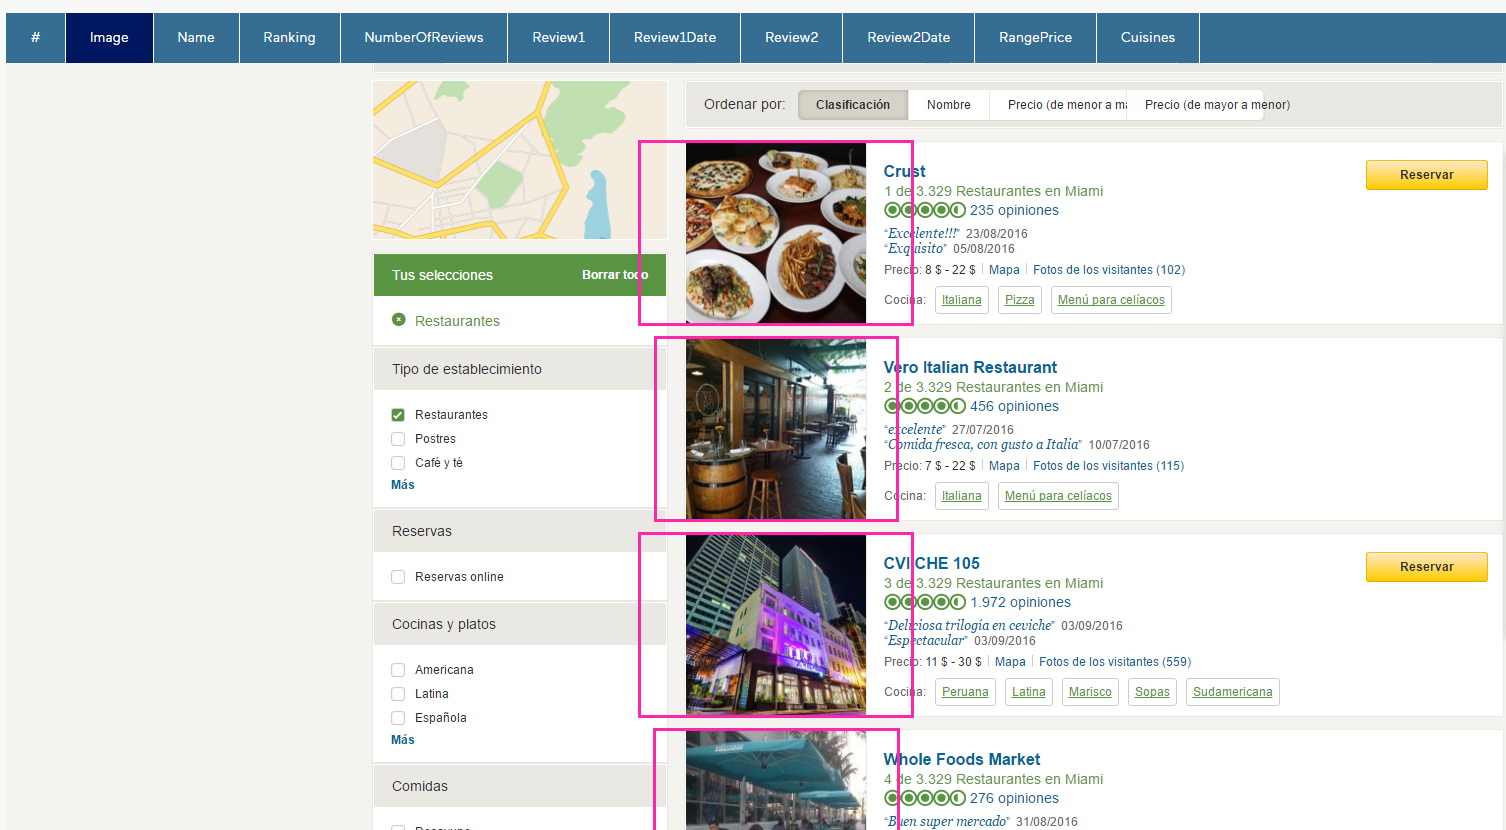
\includegraphics[width=0.8\textwidth]{./figs/ImportioEdit.png}
	\caption{Pantalla de edición de los elementos HTML a extraer en la tabla generada por import.io.}
	\label{fig:ImportioEdit}
\end{figure}

Como última característica, cabe destacar que import.io, en su versión de pago, permite la actualización automática de los cambios que se produjesen en la hoja de cálculo resultante. Es decir, en caso de que el sitio web cambiase, algo muy frecuente en sitios web de esta índole, import.io se encargaría de escanear y extraer la tabla con el formato que se haya preestablecido.

Al igual que existe import.io, existen otras herramientas para la extracción de datos en forma tabular:
\begin{itemize}
	\item \textbf{importhtml de Google Spreadsheets}\footnote{Extracción de datos con importhtml de Google SpreadSheets: \url{https://mashe.hawksey.info/2012/09/reshaping-importhtml-data-in-google-spreadsheet-using-query-and-transpose-formula/}}, menos potentes, pero mucho más sencilla de utilizar y con contenido actualizable.
	\item \textbf{Gneiss Spreadsheet} permite definir consultas y extraer datos en forma de tabla de un servicio web RESTful API \cite{Chang2014} con la funcionalidad de auto-actualización de los datos.
\end{itemize}

\chapter{Wit.ai: Procesamiento del lenguaje natural orientado a bots conversacionales}
\label{anx:witai}

Wit.ai se define como una herramienta de procesamiento del lenguaje, ya sea para texto como para voz. El objetivo de esta herramienta es funcionar de nexo entre el lenguaje que comprenden los humanos y las funcionalidades que dispone un sistema software, como lo puede ser un chatbot. Trabaja con diferentes lenguajes como el inglés o el castellano (en fase de desarrollo actualmente, aunque funciona relativamente bien). La principal virtud es que con poco trabajo Wit.ai empieza a funcionar como es esperado. Wit.ai funciona a base de entrenamiento, es decir, el desarrollador de la aplicación debe de ir introduciendo frases que el usuario utilizaría para hacer peticiones al sistema. A medida de que disponga de más frases más preciso será encontrando las intenciones (Intents) o entidades que los usuarios hayan introducido.

Respecto al trabajo referente a SheetChat, se ha delegado la tarea de desambiguación de Intents y reconocimiento de entidades a Wit.ai. Wit.ai permite tanto introducir frases de manera manual o esperar a recibir frases de los usuarios e ir corrigiendo desambiguaciones en las que se haya podido equivocar Wit.ai para mejorar su sistema de reconocimiento. En la Figura \ref{fig:WitaiInbox} se pueden observar dos mensajes introducidos por alguno de sus usuarios. El sistema ha reconocido tanto la entidad alumno como el Intent al que se refería el usuario. Sin embargo en la Figura \ref{fig:WitaiFallo} Wit.ai ha sido incapaz de obtener toda la información necesaria para resolver la pregunta del usuario. En la imagen superior ha reconocido erroneamente el Intent y no ha visto la entidad alumno (lo que indica que requiere más entrenamiento con frases de ese tipo). En la imagen inferior si ha sido capaz de reconocer adecuadamente el Intent, pero no ha podido obtener la entidad alumno, por lo que tendrá que preguntar por ella para dar respuesta al Intent.

\begin{figure}[htb]
	\centering
	\includegraphics[width=0.8\textwidth]{./figs/WitaiInbox.png}
	\caption{Wit.ai infiriendo de dos frases cuales son los Intents correspondientes para cada uno de ellos y cuál es la entidad Alumno.}
	\label{fig:WitaiInbox}
\end{figure}

\begin{figure}[htb]
	\centering
	\includegraphics[width=0.8\textwidth]{./figs/WitaiFallo.png}
	\caption{En la imagen de arriba Witai infiere erroneamente el Intent y no reconoce la entidad. En la inferior el usuario no ha proporcionado ninguna entidad, por lo que el chat tendrá que preguntar por ella.}
	\label{fig:WitaiFallo}
\end{figure}

Como se ha mencionado previamente, Wit.ai funciona en base a una confianza en las detecciones que ha hecho. En SheetChat se exige que el grado de confianza ha de ser mayor que 0.5 sobre 1 para que una inferencia se de por válida. En la Figura \ref{fig:WitaiConfianza} se puede observar como el grado de confianza de que \emph{María} es un alumno es de 0.99 y que el Intent es \emph{fisicaPonderadaPorEjercicio} únicamente de 0.71. Si se le ha entrenado adecuadamente, es muy probable que María sea un alumno y, con una confianza menor, que lo que se quiere es obtener la media ponderada de los ejercicios de física.

\begin{figure}[htb]
	\centering
	\includegraphics[width=0.8\textwidth]{./figs/WitaiConfianza.png}
	\caption{Respuesta del servicio de wit.ai cuando se le proporciona una frase. Remarcado en morado está el grado de confianza referente a la entidad alumno que ha detectado, de azul la del Intent.}
	\label{fig:WitaiConfianza}
\end{figure}




























% line in order to check if utf-8 is properly configured: áéíóúñ

